\chapter{Memory Bank Prioritization}\label{ch5}
\noindent
In the previous chapter, we have discussed about the methods to evaluate the optimal number of memory banks required to design
a mixed-criticality system. Also, given a mixed-criticality system with t number of tasks, whether a memory with n number of 
banks can support such a system can also be evaluated by solving an ILP discussed in the previous chapter. With the help of
the methods explained in the previous chapter, for a particular mixed criticality-system, we can get a schedule which 
determines which task should be executed at which criticality level/mode in every cycle so that the mixed-criticality system 
can be executed with the given memory system. 
\newline
\newline
Each critical task in the mixed-criticality system consists of multiple memory requests and number of parallel memory bank
access at each criticality level. The computation to determine the optimal number of banks for the design of such a 
mixed-criticality system is evaluated offline. The main disadvantage of this method is that the memory requests may not always 
allow parallel bank access when requests are served in real systems. After address translation, two or more memory requests 
may get mapped to same bank. Again, due to the open row policy, discussed in the introductory chapters, some memory requests 
get prioritized over the other. This problem have been discussed in the next section with the help of an example.

\section{Motivating Example}
\noindent
Consider a mixed-criticality system consisting of two tasks with 5 and 8 memory requests respectively. The tasks specifications 
are shown in Table \ref{tab7}. It has been found that to execute the tasks within their deadlines we need a memory with 
atleast 3 banks. Each bank is assumed to be of size 128B with row size of 16B. So each bank has 8 rows. Each row again consists 
of 4 columns of 4B each. The memory is word addressable, so each address is of 4B. The address mapping of each bank is 
given below -
\begin{description}
 \item {\bf Bank 0}: Address 0-31 is mapped on this bank. Each row consists of 4 addresses, address 0-3 maps to row 0 of Bank 0, 
 similarly address 4-7 maps to row 1 of Bank 0.
 \item {\bf Bank 1}: Address 32-63 is mapped on this bank. Address 32-35 is mapped to row 0 of Bank 1. Similarly, address 60-63 is 
 mapped to row 7 of Bank 1.
 \item {\bf Bank 2}: Address 64-95 is mapped on this bank. Address 64-67 is mapped to row 0 of Bank 2. Similarly, address 91-95 is
 mapped to row 7 of Bank 2.
\end{description}

Now when these tasks are allowed to execute, the memory addresses generated by the above tasks are listed in
Table \ref{tab8}. If we schedule the above tasks according to the optimal schedule generated by ILP, we need to execute 
the tasks in the following sequence in every cycle -

\begin{table}[t]
\centering
\begin{tabular}{|c|c|c|c|c|c|}\hline
 Task ID & Criticality & Parallel Bank  & Percentage of & Deadline \\
         & Level & Access  & task executed &  \\ \hline
 1 & L1 & 1 & 20\% & 4 \\ 
   & L2 & 2 & 40\% & \\
   & L3 & 3 & 60\% & \\ \hline
 2 & L1 & 1 & 12.5\% & 6 \\
   & L2 & 2 & 25\% & \\
   & L3 & 4 & 50\% & \\ \hline
\end{tabular} 
\caption{Task Specifications}
\label{tab7}
\end{table}

 
\begin{description}
 \item {\bf Cycle 1}: T1 executes in Criticality level 1 with one bank access. T2 executes in Criticality level 2 with 2 
 parallel bank access. So in Cycle 1 we require 3 parallel bank accesses. 
 \item {\bf Cycle 2}: T1 executes in Criticality level 2 with two parallel bank access. T2 executes in Criticality level 1 
 with one bank access. So, in Cycle 2, we have 3 parallel bank accesses.
 \item {\bf Cycle 3}: T1 executes in Criticality level 2 with 2 parallel bank access. T2 executes in Criticality level 1
 with one bank access. So, we have 3 parallel bank accesses in Cycle 3.
 \item {\bf Cycle 4}: T2 executes in Criticality level 2 with 2 parallel bank accesses.
 \item {\bf Cycle 5}: T2 executes in Criticality level 2 with 2 parallel bank accesses. 
\end{description}



\begin{table}[t]
 \begin{tabular}{|c|c|c|c|c|}\hline
 Task ID & Number of & Memory Addresses & Bank Number & Row Number\\ 
         & Memory Requests &            &             &            \\ \hline
 1 & 5 & 12 & 0 & 3 \\
   &   & 36 & 1 & 1 \\
   &   & 15 & 0 & 3 \\
   &   & 39 & 1 & 1 \\
   &   & 42 & 1 & 2 \\ \hline
 2 & 8 & 10 & 0 & 2 \\
   &   & 22 & 0 & 5 \\
   &   & 66 & 2 & 0 \\
   &   & 37 & 1 & 1 \\
   &   & 72 & 2 & 2 \\
   &   & 75 & 2 & 2 \\
   &   & 79 & 2 & 3 \\
   &   & 83 & 2 & 4 \\ \hline   
 \end{tabular}
\caption{Memory Address Mapping}
\label{tab8}
\end{table}

After address translation, the mapping of different requests on different memory banks is explained below.
\newline
\newline
{\bf Explanation}: In cycle 1, Row 3 of Bank 0 (address 12) is brought in the rowbuffer of Bank 0. Row 2 of Bank 0
 (address 10) and Row 5 of Bank 0 (address 22) though scheduled to be served in Cycle 1, but cannot be served as some other
 request from T1 has already been scheduled to be served in the rowbuffer of Bank 0. So these two requests are kept in the 
 waiting queue to be served later. 
\newline
\newline
In cycle 2,  Row 1 of Bank 1 (address 36) is brought to the rowbuffer of Bank 1. Row 3 of Bank 0 (address 15) results in row 
hit in Bank 0. So memory request to access address 15 is prioritized over pending requests to access address 10 and address 22.
Thus, address 15 is served first. Similarly, in Cycle 3, request corresponding to address 39 is prioritized over other 
pending requests as address 39 is mapped to Row 1 of Bank 1 which is already in rowbuffer of Bank 1. 
\newline
\newline
Table \ref{tab9} shows in detail the overview of memory in every cycle. After address mapping of several memory requests to 
different memory banks, it has been found that both T1 and T2 fails to meet their deadline when executed on a memory with 
2 banks.

\begin{table}[t]
 \begin{tabular}{|c|c|c|c|c|}\hline
 Cycle & Incoming & Previous Pending & Requests Served in & Deadline \\ 
       & Requests  & Requests         & the current cycle & Miss \\ \hline      
 1 & 12 (Bank 0, Row 3) & & 12 (Bank 0, Row 3) &  \\ 
   & 10 (Bank 0, Row 4) & & & \\ 
   & 22 (Bank 0, Row 5) & & & \\ \hline
 2 & 36 (Bank 1, Row 1) & 10 (Bank 0, Row 4) & 15 (Bank 0, Row 3) & \\ 
   & 15 (Bank 0, Row 3) & 22 (Bank 0, Row 5) & 36 (Bank 1, Row 1) & \\
   & 66 (Bank 2, Row 0) &                    & 66 (Bank 2, Row 0) & \\ \hline
 3 & 39 (Bank 1, Row 1) & 10 (Bank 0, Row 4) & 10 (Bank 0, Row 4) & \\
   & 42 (Bank 1, Row 2) & 22 (Bank 0, Row 5) & 39 (Bank 1, Row 1) & \\
   & 37 (Bank 1, Row 1) &                    &                    & \\ \hline
 4 & 72 (Bank 2, Row 2) & 22 (Bank 0, Row 5) & 22 (Bank 0, Row 5) & \\
   & 75 (Bank 2, Row 2) & 37 (Bank 1, Row 1) & 37 (Bank 1, Row 1) & \\ 
   &                    &                    & 72 (Bank 2, Row 2) & \\ \hline
 5 & 79 (Bank 2, Row 3) & 75 (Bank 2, Row 2) & 75 (Bank 2, Row 2) & T1\\ 
   & 83 (Bank 2, Row 4) &                    &                    & \\ \hline
 6 &                    & 79 (Bank 2, Row 3) & 79 (Bank 2, Row 3) &  \\ 
   &                    & 83 (Bank 2, Row 4) &                    &  \\ \hline
 7 &                    & 83 (Bank 2, Row 4) &                    & T2 \\ \hline
 \end{tabular}
\caption{Overview of Memory from cycle to cycle}
\label{tab9}
\end{table}

\section{Disadvantage of the existing method}\label{dotam}
\noindent
The main disadvantage of the existing method is due to the address mapping policy, many requests get mapped to same bank and 
hence get buffered in the waiting queue. They have to wait for the bank availability in the subsequent cycles. When a memory
address is served, the row to which this address belongs is brought to the rowbuffer in the memory. The memory request is 
then served by reading/writing at the appropriate column in that row in the rowbuffer. On the next cycle, if some memory 
request arrives which maps to the same bank and same row in the rowbuffer, the address is served first though some other 
addresses are waiting for memory access in the waiting queue. Due to this phenomenon, some tasks miss their deadlines in spite
of waiting for cycle in the waiting queue. 

\section{Hardness Characterisation of the problem}\label{hcotp}
\noindent
\begin{problem}
 Given a set of $n$ memory requests (M1, M2, M3 $\dots$ Mn) coming from a set of k tasks having different deadlines
 (D1, D2, $\dots$ Dk), executing on a memory with m banks. Can we schedule $n$ memory requests on m banks over $T$ cycles based 
 on the address to which they are mapped so that all $t$ tasks can meet their deadlines.
\end{problem}

\noindent
The problem is NP-complete.
\newline
\newline
The problem is in NP.
\newline
\newline
Given a schedule to serve $n$ memory requests, whether all $n$ memory requests corresponding to $t$ tasks can be executed over $T$ 
cycles can be verified in polynomial time.
\newline
\newline
The problem is NP-hard.
\newline
\newline
To show that our problem is NP-hard, we give a polynomial time reduction from CNF-SAT problem~\cite{wiki:xxx8} to our problem.
Given an instance $\alpha$ of CNF-SAT problem, we will generate an instance of our problem $\sigma$ such that if $\alpha$
is satisfiable, $\sigma$ can serve $n$ memory requests over $T$ cycles within the individual task deadlines. 
\newline
\newline
Our problem can be considered as a variant of the CNF-SAT problem~\cite{wiki:xxx8}. In Boolean logic, a formula is in conjunctive normal 
form (CNF) or clausal normal form if it is a conjunction of clauses, where a clause is a disjunction of literals, otherwise 
put, it is an AND of ORs. $n$ memory requests get mapped to m different banks based on the address of each request. At a 
particular instant, a bank may remain free, whereas, many requests may get buffered at some other bank. We can think of $n$ 
memory requests as a set of $n$ clauses. We can think of our problem C as a set of $n$ clauses ${C_{1},C_{2},C_{3},\dots C_{n}}$.
$i^{th}$ clause, $C_{i}$ is True, if $i^{th}$ memory request gets served within the task deadline, otherwise, $C_{i}$ is False.
Our goal is to give an assignment to the variables $\sigma$ : V $\rightarrow$ {True, False} so that C evaluates to True.
So, if $\alpha$ is satisfiable, $\sigma$ can serve $n$ memory requests over $T$ cycles within the task deadlines.
\newline
\newline
The converse is also true.
\newline
\newline
Given $\sigma$ can execute $n$ memory requests within their deadlines. This indicates that all the memory requests can be served 
within the task deadlines over $T$ cycles. Now, when $i^{th}$ task gets executed within the task deadline, $C_{i}$ is assigned 
True. So, if all $n$ memory requests get served within the task deadlines, then $C_{i}$ is assigned True, where i varies from 1 
to n. Thus, C becomes satisfiable. So, if $\sigma$ can complete execution of $n$ memory requests within the task deadlines, 
$\alpha$ becomes satisfiable.
\newline
\newline
Thus, whether a set of $n$ memory requests from $t$ tasks can be served within individual task deadlines is NP-complete.


\section{Solution to the problem}\label{sttp}
\noindent
To solve the above problem, we propose a novel bank aware address mapping heuristic which partitions the memory requests based on 
a gain function calculated locally on arrival of a memory request. We use a partitioning heuristic to partition the memory requests across banks. 

\subsection{Bank scheduling using Task partitioning}\label{FM}
\noindent
We use an iterative heuristic for partitioning the network whose worst case computation time per pass 
grows linearly with size of the network~\cite{fiduccia1988linear} and which in general converges after several passes. 
Generally, very small number of passes are needed leading to a fast approximation algorithm for mincut partitioning, which is the basis of our work.  
\newline
\newline
Given a network consisting of a set of cells(modules) connected by a set of nets(signals), the mincut partitioning problem
consists of finding a partition of the set of cells into two blocks A and B such that the number of nets in the block is 
minimum. This is the main objective of our algorithm. 

\subsection{Our proposed methodology}\label{mfm}
\noindent
Consider a mixed-criticality system where n is the optimal number of banks required to design such a system. We suggest to 
keep two extra banks which will not participate in address mapping. These two extra banks will be used to serve the pending 
requests in the waiting queue so that we can minimize the deadline misses of tasks. We consider the memory requests as the 
nodes in our problem. Requests which are mapped to same bank form a partition. We start with an initial partition of 
requests, which makes up our initial partition. We calculate a gain function over the task as the difference in the gains 
achieved by serving a memory request in the same bank or in some reserved bank. This difference in the two gains helps to 
decide whether a memory request will be served inplace or in the reserved bank. Gain function can be explained formally as -
\newline
\newline
Gain($Req_{i}$) = Gain(Serving $Req_{i}$ in the same bank) - Gain(Serving $Req_{i}$ in some reserved bank)
\newline
\newline
= [T.deadline - (total memory access time + total waiting time in existing method)] - [T.deadline - (total memory access time 
+ total waiting time in our method)]
\newline
\newline
Here, T is the task whose memory request is being served and T.deadline is the deadline of the task T.
Let us consider that the $i^{th}$ memory request $Req_{i}$ has been mapped to $j^{th}$ row ($Row_{j}$) of $k^{th}$ bank 
($Bank_{k}$). There are few cases with the help of which we can highlight the above problem.
\begin{description}
 \item {\bf Case 1}: If the rowbuffer of $Bank_{k}$ currently holds the $Row_{j}$ and if no other request is found to be 
 mapped to $Row_{j}$, then the $Req_{i}$ will be served immediately. So we do not need to replace $Req_{i}$. The cost to 
 serve $Req_{i}$ is equal to 1 row access time.
 
 \item {\bf Case 2}: If $p$ number of requests all mapping to different rows of same bank, are ahead of $Req_{i}$ in the 
 waiting queue, then according to the FR-FCFS 
 policy, $Req_{i}$ will be served after $p$ requests. In this case, if the cost to serve $Req_{i}$ in any one of the reserved 
 banks is greater than that to solve after $p$ memory requests of same bank, we allow $Req_{i}$ to be served in $Bank_{k}$.
 So the cost to serve $Req_{i}$ is the total time to serve $p$ row misses followed by 1 row miss time. On the other hand, 
 if $p'$ out of $p$ requests map to the same bank as the rowbuffer, then $Req_{i}$ will be served after $p'$ row hits
 followed by $p - p'$ row misses. 
 
 \item {\bf Case 3}: If the rowbuffer of $Bank_{k}$ currently holds some row other than $Row_{j}$, say $Row_{j'}$, and if 
 say $k'$ number of requests are infront of $Req_{i}$ in the waiting queue, then we need to calculate the cost to serve 
 $Req_{i}$ in $Bank_{k}$ after serving $k'$ requests. Considering all $k'$ requests result in row miss, the time to serve 
 $Req_{i}$ is the total time to serve $k'$ row misses followed by 1 row miss corresponding to $Req_{i}$. We need to calculate 
 the cost to serve $Req_{i}$ in any reserved bank, say $Res_{l}$. To serve $Req_{i}$ in any reserved bank, $Res_{l}$, we need 
 to copy $Row_{j}$ of $Bank_{k}$ to any row, say $l'$ of $Res_{l}$ and bring that row in the rowbuffer. So the total time to 
 serve $Req_{i}$ is the time to copy $Row_{j}$ to $Res_{l}$ followed by the time to bring the $Row_{j}$ to the rowbuffer.  
\end{description}

\noindent
If the difference of the two costs in the Gain function is greater than 0, we serve $Req_{i}$ in $Bank_{k}$, otherwise, we 
serve $Req_{i}$ in one of the reserved banks. 

\subsection{Algorithm for Bank Aware partitioning}\label{bafm}
Algorithm \ref{alg4} explains Bank Aware partitioning. We give a detailed explanation of our algorithm. Our algorithm takes
as input a memory request of a task T in the form of $<address, request type>$, number of parallel memory accesses of the task 
T that are left to be scheduled and deadline of the task as input to our algorithm. Our output is the bank number to which each address will get mapped. 
\newline
\newline
{\bf Step 1}: The bank to which the Req is mapped is evaluated. The variable Bank is assigned that value. n is 
assigned the number of requests ahead of Req in the waiting queue.
\newline
{\bf Step 2}: The number of requests in the waiting queue which are mapped to the same bank and same row as the Req is 
calculated. n2 is assigned that value. The number of requests which are mapped to some other bank other than Bank is calculated 
and n3 is assigned that value.
\newline
{\bf Step 3}: If the row of the Req is same as that in the rowbuffer of the Bank, then we calculate the waiting time of Req.
Three cases can occur-
\newline
Case 1: n2 = 0, then the waiting time of Req is $wait\_time_{1}$ =  0.
\newline
Case 2: n2 = n, then the waiting time of Req is $wait\_time_{1}$ = n * t1, where t1 is the memory access time when there is a row hit.
\newline
Case 3: n2 $>$ 0 and n2 $<$ n, then the waiting time of Req is the time to serve n2 row hits followed, ie,$wait\_time_{1}$ =
n2*t1. 
\newline
{\bf Step 4}: If the row of the Req is not the same as that in the rowbuffer of the Bank, then the waiting time 
of Req, $wait\_time_{1}$ = n2*t1 + (n - n2 - n3)*t2, where t2 is the memory access time when there is a row miss.
\newline
{\bf Step 5}: The waiting time of Req if served in any one of the reserved memory bank is $wait\_time_{2}$ = t3, where t3 includes the time to 
copy a row from one bank to another and the time to bring the copied row to the rowbuffer of the reserved memory bank.
\newline 
{\bf Step 6}: We calculate gain in the above two methods. Gain by method 1 is given as $Gain_{1}$ = deadline - ($wait\_time_{1}$ 
+ n1*M), where M is the worst case memory access time. Gain by method 2 is given as $Gain_{2}$ = deadline - ($wait\_time_{2}$ 
+ n1*M). 
\newline
{\bf Step 7}: If $Gain_{1}$ is greater than $Gain_{2}$, then we serve the request in Bank, otherwise we serve the memory 
request in any reserved memory bank.




\begin{algorithm}
 \caption{\bf Bank Aware Partitioning(Req, n1, deadline)}
  \begin{algorithmic}[1]
  \State {\bf Input} Req: Memory request to be served, n1: number of pending parallel accesses, deadline: deadline of the task
  \State {\bf Output} Bn : Bank number on which Req is finally scheduled
  \State t1 = memory access time when row hit
  \State t2 = memory access time when roow miss
  \State t3 = time to copy a row to the Reserved Bank
  \State M = Worst Case memory access time
  \State n = number of requests in the waiting queue before task T
  \State Bank = Req.bank \Comment Bank to which Req is initially mapped
  \State n2 = 0
  \State n3 = 0
  \For {i = 1 to n}
  \If {$Req_{i}.bank == Bank$}\Comment checks if some other request is mapped to the same bank as Req
  \If {$Req_{i}$.row == Bank.rowbuffer}\Comment checks if some other request is mapped to the same row as Req 
  \State n2 = n2 + 1
  \EndIf
  \Else
  \State n3 = n3 + 1
  \EndIf
  \EndFor
  \If {Req.row == Bank.rowbuffer}
   \If {n2 == 0}
   \State $wait\_time{1}$ = 0
   \ElsIf {n2 $>$ 0 and n2 $<$ n1}
   \State $wait\_time{1}$ = n2 * t1 
   \ElsIf {n2 == n} 
   \State $wait\_time{1}$ = n * t1 
   \EndIf
  \ElsIf {Req.row $\neq$ Bank.rowbuffer}
   \State $wait\_time{1}$ = n2 * t1 + (n - n2 - n3) * t2 
  \EndIf
  \State $wait\_time{2}$ = t3 
  \State $Gain_{1}$ = Task.deadline - ($wait\_time_{1}$ + $n1 * M$)
  \State $Gain_{2}$ = Task.deadline - ($wait\_time_{2}$ + $n1 * M$)
  \If {$Gain_{1}$ $>$ $Gain_{2}$}
  \State Bn = Bank.row 
  \Else
  \State copy Bank.row to any row in the Reserved bank
  \State Bn = Reserved.row
  \EndIf
  \State return Bn
  \end{algorithmic}
\label{alg4}
\end{algorithm}

\subsection{Solution with an Example}\label{swae}
\noindent
Consider the same set of tasks as in Table \ref{tab7} and Table \ref{tab8} respectively. The above discussed method when 
applied on the same set of tasks with same memory requests, generates the following result as in Table \ref{tab10}. We have 
assumed that the time to serve each memory request is 1 cycle. We have assumed that our system in this example has one extra 
reserved memory bank denoted by Res. It has been found that on adopting our method, both T1 and T2 can be served within their 
deadlines.

\begin{table}[t]
 \begin{tabular}{|c|c|c|c|c|}\hline
 {\bf Cycle} & {\bf Incoming} & {\bf Previous Pending} & {\bf Requests Served in} & {\bf Deadline} \\ 
       & {\bf Requests}  & {\bf Requests}         & {\bf the current cycle} & {\bf Miss} \\ \hline      
 1 & 12 (Bank 0, Row 3) & & 12 (Bank 0, Row 3) &  \\ 
   & 10 (Bank 0, Row 4) & & & \\ 
   & 22 (Bank 0, Row 5) & & & \\ \hline
 2 & 36 (Bank 1, Row 1) & 10 (Bank 0, Row 4) & 15 (Bank 0, Row 3) & \\ 
   & 15 (Bank 0, Row 3) & 22 (Bank 0, Row 5) & 36 (Bank 1, Row 1) & \\
   & 66 (Bank 2, Row 0) &                    & 66 (Bank 2, Row 0) & \\ \hline
 3 & 39 (Bank 1, Row 1) & 10 (Bank 0, Row 4) & 10 (Bank 0, Row 4) & \\
   & 42 (Bank 1, Row 2) & 22 (Bank 0, Row 5) & 39 (Bank 1, Row 1) & \\
   & 37 (Bank 1, Row 1) &                    &                    & \\ \hline
 4 & 72 (Bank 2, Row 2) & 22 (Bank 0, Row 5) & 22 (Bank 0, Row 5) & \\
   & 75 (Bank 2, Row 2) & 37 (Bank 1, Row 1) & 37 (Bank 1, Row 1) & \\ 
   &                    &                    & 72 (Bank 2, Row 2) & \\ 
   &                    &                    & 42 (Res 0, Row 2)  & \\ \hline
 5 & 79 (Bank 2, Row 3) & 75 (Bank 2, Row 2) & 75 (Bank 2, Row 2) & \\ 
   & 83 (Bank 2, Row 4) &                    &                    & \\ \hline
 6 &                    & 79 (Bank 2, Row 3) & 79 (Bank 2, Row 3) &  \\ 
   &                    & 83 (Bank 2, Row 4) & 83 (Res 0, Row 4)  &   \\ \hline
 7 &                    &                     &                   &  \\ \hline
 \end{tabular}
\caption{Overview of Memory from cycle to cycle on using Bank Aware Partitioning}
\label{tab10}
\end{table}


\subsection{Performance Analysis}\label{opom}
\noindent
Consider two memory requests, $M_{1}$ arriving at instant $t_{1}$ and $M_{2}$ arriving at instant $t_{2}$, where $t_{1}$ $<$ 
$t_{2}$. Let $M_{1}$ and $M_{2}$ are mapped to the same Bank $B$ at rows $R_{1}$ and $R_{2}$ respectively. 
Let $R$ be the active row in the rowbuffer of bank $B$. If $R_{1}$ = $R$, then $M_{1}$ will be served first followed by 
$M_{2}$. But if $R_{2}$ = $R$, then $M_{2}$ will be served first due to open row policy, followed by $M_{1}$.
\newline
\newline
Now, consider there be $n$ requests arriving after $M_{2}$, all mapping to the same row $R$. According to the open row policy,
all the n requests will be served first, then $M_{2}$ will be served. Let $\tau_{1}$ units be the time to execute a memory 
request if there is a row hit. Let $\tau_{2}$ units be the time to execute a memory request if there is a row miss. Clearly, 
$\tau_{2}$ $>$ $\tau_{1}$. $\tau_{1}$ includes only row access time, whereas, $\tau_{2}$ includes loading of a row to the 
rowbuffer of a bank followed by row access time. So, $M_{2}$ will get a chance to execute after ($n$ * $\tau_{1}$ + $\tau_{2}$)
units. Let $M_{2}$ has arrived from Task $T$ whose deadline is given by $T.deadline$ units. Let $X$ be the number of parallel 
accesses remaining to be served in the memory after $M_{2}$ gets served. Now, the Gain of $M_{2}$ by following the 
conventional method for scheduling in DRAM, denoted by 
$Gain_{1}(M_{2})$ is given by - 
\newline
\newline
$Gain_{1}(M_{2})$ = $T.deadline$ - ($n$ * $\tau_{1}$ + $\tau_{2}$ + $X$ * $\alpha$)
\newline
\newline
where $\alpha$ is the maximum memory access time to execute an instruction,
\newline
\newline
Let $\tau_{3}$ be the time to copy a row from Bank $B$ to one of the reserved bank $R_{b}$. Following our method, the Gain of 
$M_{2}$, denoted by $Gain_{2}(M_{2})$ is given by -
\newline
\newline
$Gain_{2}(M_{2})$ = $T.deadline$ - ($\tau_{3}$ + $\tau_{1}$ + $X$ * $\alpha$)
\newline
\newline
If $Gain_{2}(M_{2})$ $>$ $Gain_{1}(M_{2})$, we follow our method. Otherwise, we follow the existing method. 
\newline
\newline
$Gain_{2}(M_{2})$ - $Gain_{1}(M_{2})$ $>$ 0
\newline 
\newline
$\implies$ [$T.deadline$ - ($\tau_{3}$ + $\tau_{1}$ + $X$ * $\alpha$)] - [$T.deadline$ - ($n$ * $\tau_{1}$ + $\tau_{2}$ + $X$ * $\alpha$)] $>$ 0
\newline
\newline
$\implies$ $n$ * $\tau_{1}$ + ($\tau_{2}$ - $\tau_{1}$) - $\tau_{3}$ $>$ 0
\newline
\newline
$\implies$ $n$ * $\tau_{1}$ - $\tau_{3}$ $>$ 0 [Since, $\tau_{2}$ - $\tau_{1}$ $>$ 0]
\newline
\newline
when n is very large, $n$ * $\tau_{1}$ $>>$ $\tau_{2}$
\newline
\newline
So, $Gain_{2}(M_{2})$ - $Gain_{1}(M_{2})$ $>$ 0. 
\newline
Hence, our method is expected to yield better results than the conventional open row strategy. 
Further, we discuss the advantages of our method over existing method. 
\newline
\newline
 {\bf 1. Requests mapping to two different rows in the same bank in an interleaved manner - } 
 \newline
 \newline
 Let $\alpha_{1}, \alpha_{2}, \dots \alpha_{n}$ be $n$ memory requests mapping to bank B in such a manner that all 
 $\alpha_{2i}$ are mapped to row R1 and all $\alpha_{2i + 1}$ are mapped to row R2 of B. If the rowbuffer of bank B holds 
 row R1, then all odd requests will be pending in the waiting queue, whereas all even requests will get served. So, by open 
 row policy, there will be n/2 row misses. Now, if we apply our method, row R2 will be mapped to some reserved bank in the 
 system, say B' and all the odd requests will be directed to bank B' and served in that bank. So, we can increase the 
 probability to meet the deadlines of the tasks.
 \newline
 \newline
 {\bf 2. Two critical tasks from two critical applications accessing two different chunks of memory mapped in consecutive 
 locations - }
 \newline
 \newline
 Let us consider two critical tasks from two different applications are accessing memory locations in such a way that task
 from the first application are all mapped to row R1 of bank B, whereas, task from the second application are mapped to 
 row R2 of bank B. Following the existing policy, either one of the tasks can meet their deadlines. The other task from the 
 second application will not be able to meet their deadlines. Following our proposed method, the row from the second task
 will be copied to the reserved bank and all the remaining requests corresponding to that row get diverted to the reserved 
 bank and meet deadline of both the tasks from different applications.
 

\section{Results}\label{res2}
This section deals with our discussions on implementation, benchmark programs used by us and results obtained from normal DRAMs
vs our modified DRAM controller. We have implemented our own simulator. We have generated our results on Malardalen WCET
benchmarks ~\cite{gustafsson2010malardalen}. Table ~\ref{tab11} gives a a description of the benchmark programs. We have 
generated our memory trace on these benchmark programs. Table \ref{tab12} gives a description of some of the tasksets 
which are generated based on the number of instructions in the memory traces. We have compared the performances of our 
modified DRAM controller with existing DRAM controllers on a memory with bank of size 32B and 64B respectively. 
Some of the results have been shown in Table ~\ref{tab13}.

\begin{table}
 \begin{tabular}{|c|c|c|}\hline 
 {\bf Benchmark Program} & {\bf Number of Instructions} & {\bf Memory Instructions} \\ \hline
 bs.c & 179 & 64 \\ \hline
 cnt.c & 295 & 95 \\ \hline 
 duff.c & 257 & 111 \\ \hline
 fac.c & 164 & 48 \\ \hline
 fibcall.c & 163 & 55 \\ \hline
 insertsort.c & 189 & 66 \\ \hline
 lcdnum.c & 198 & 49 \\ \hline
 ns.c & 245 & 71 \\ \hline
 prime.c & 227 & 69 \\ \hline
 \end{tabular}
\caption{Details of Malardalen WCET benchmark programs}
\label{tab11}
\end{table}



\begin{table}
{\centering
 \begin{tabular}{|c|c|c|c|c|}\hline
  {\bf Dataset}  & {\bf Benchmark} & {\bf criticality} & {\bf number of parallel} & {\bf percentage of}\\ 
  {\bf Number}  &  {\bf program}   &  {\bf level}      & {\bf accesses}  & {\bf task completed}  \\ \hline
  Dataset I & fibcall.c & L1 & 3 & 6\% \\
            &           & L2 & 4 & 8\%       \\
            &            & L3 & 6 & 12\%           \\
            & lcdnum.c & L1 & 2 & 3\%    \\
            &          & L2 & 3 & 5\%     \\
            &          & L3 & 4 & 7\%          \\
            & fac.c & L1   &  1  & 2\%   \\
            &       & L2   &  2  & 4\%    \\
            &       & L3   & 4   & 8\%   \\ \hline 
 Dataset II & bs.c & L1  & 5  & 7\% \\
            &      & L2  & 8  & 12.5\% \\
            &      & L3 & 10 & 15\% \\
            & cnt.c & L1 & 5 & 5\%\\
            &       & L2 & 7 & 7\%     \\
            &       & L3 & 10 & 10\%    \\
            & duff.c & L1 & 7 & 6\% \\
            &        & L2 & 9 & 8\% \\
            &        & L3 & 11 & 9\% \\ \hline
 Dataset III & prime.c & L1 & 3 & 4\% \\
             &         & L2 & 6 & 8\% \\
             &         & L3 & 9 & 13\% \\
             & ns.c & L1 & 4 & 5\% \\
             &      & L2 & 6 & 8\% \\ 
             &      & L3 & 10 & 14\% \\
             & insertsort.c & L1 & 3 & 4\% \\
             &              & L2 & 6 & 9\% \\
             &              & L3 & 8 & 12\% \\ \hline
 Dataset IV  & lcdnum.c & L1 & 5 & 10\% \\
             &          & L2 & 7 & 14\% \\
             &          & L3 & 9 & 18\% \\
             & insertsort.c & L1 & 6 & 9\% \\
             &              & L2 & 8 & 12\% \\
             &              & L3 & 10 & 15\% \\
             & fibcall.c & L1 & 5 & 9\% \\
             &           & L2 & 8 & 14\% \\
             &           & L3 & 11 & 20\% \\ \hline
 \end{tabular}
 }
 \caption{Some Dataset generated on different benchmark programs}
 \label{tab12}
\end{table}




\begin{table}
\centering
 \begin{tabular}{|c|c|c|c|c|c|}\hline
 {\bf Dataset} & {\bf Number of} & {\bf Number of} & {\bf Rowsize} & {\bf Number of Task Miss} & {\bf Number of Task}\\
 {\bf Number}  &  {\bf cycles} & {\bf Banks} & & {\bf (conventional method)}& {\bf Miss(our method)}\\ \hline
 Dataset I & 10,000 & 10 banks & 64B & 1 & 1 \\
           & 20,000 &          &     & 3 & 2 \\
           &30,000 &          &      & 4 & 3 \\
           &40,000 &          &      & 6 & 4 \\
           & 50,000 &        &       & 8 & 5 \\
           & 60,000 &        &      & 9 & 6 \\
           & 70,000 &        &      & 11 & 7 \\ \hline
           & 10,000 & 10 banks & 32B & 2 & 1 \\ 
           & 20,000 &        &       & 4 & 2 \\
           & 30,000 &        &       & 5 & 3 \\
           & 40,000 &        &       & 8 & 5 \\
           & 50,000 &        &       & 11 & 6 \\
           & 60,000 &        &       & 12 & 7 \\
           & 70,000 &        &       & 14 & 9 \\ \hline
 Dataset II & 10,000 & 19 banks & 64B & 3 & 0 \\
            & 20,000 &         &      & 6 & 1 \\
            & 30,000 &         &      & 9 & 1 \\
            & 40,000 &         &      & 14 & 4 \\ \hline
            & 10,000 & 19 banks & 32B & 3 & 2 \\
            & 20,000 &          &     & 5 & 3 \\
            & 30,000 &          &     & 8 & 6 \\
            & 40,000 &          &     & 13 & 11 \\ \hline
 Dataset III & 10,000 & 15 banks & 64B & 2 & 1 \\
             & 20,000 &          &     & 4 & 1 \\
             & 30,000 &          &     & 5 & 2 \\
             & 40,000 &          &     & 8 & 3 \\ \hline
             &10,000 & 15 banks & 32B & 3 & 2 \\  
             & 20,000&          &     & 5 & 3 \\
             & 30,000&          &     & 6 & 4 \\
             & 40,000&          &     & 9 & 6 \\ \hline
 Dataset IV  & 10,000& 12 banks & 64B & 2 & 1 \\
             & 20,000 &         &     & 5 & 2 \\
             & 30,000 &         &     & 7 & 4 \\
             & 40,000 &         &     & 12 & 4 \\ \hline
             &10,000 & 12 banks & 32B & 3 & 2 \\
             & 20,000 &         &     & 6 & 4 \\
             & 30,000 &         &     & 9 & 6 \\
             & 40,000 &         &     & 14 & 11\\ \hline  
 \end{tabular}
\caption{Results on some of the Datasets}
\label{tab13}
\end{table}


\begin{figure}
%\label{fig1}
\centering
\fbox{
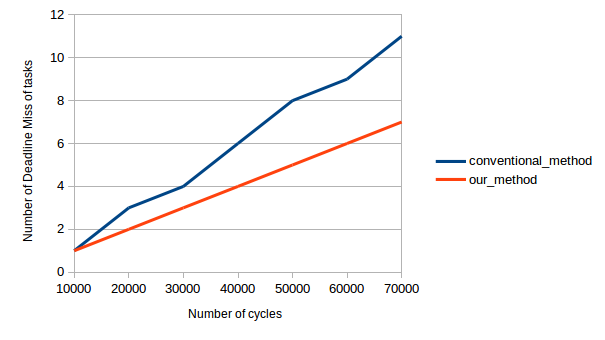
\includegraphics[width=12cm,height=7cm]{Graph_1.png}
}
\caption{Number of Task Misses on Dataset I for a memory with 10 banks and row size 64B over 70,000 cycles}
\end{figure}



\begin{figure}
%\label{fig1}
\centering
\fbox{
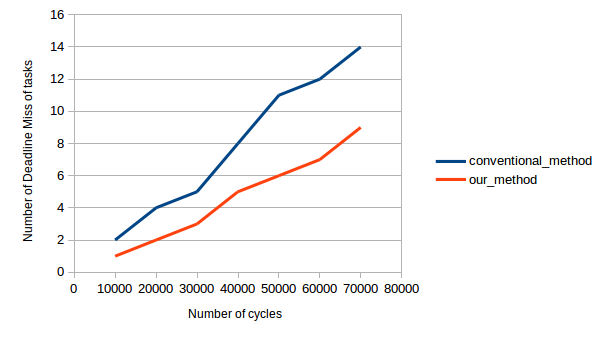
\includegraphics[width=12cm,height=7cm]{Graph_2.png}
}
\caption{Number of Task Misses on Dataset I for a memory with 10 banks and row size 32B over 70,000 cycles}
\end{figure}

\begin{figure}
%\label{fig1}
\centering
\fbox{
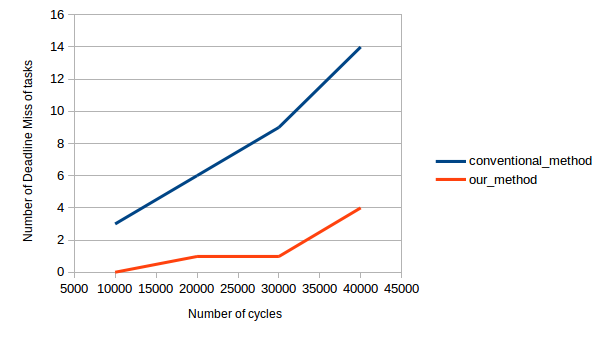
\includegraphics[width=12cm,height=7cm]{Graph_3.png}
}
\caption{Number of Task Misses on Dataset II for a memory with 19 banks and row size 64B over 40,000 cycles}
\end{figure}

\begin{figure}
%\label{fig1}
\centering
\fbox{
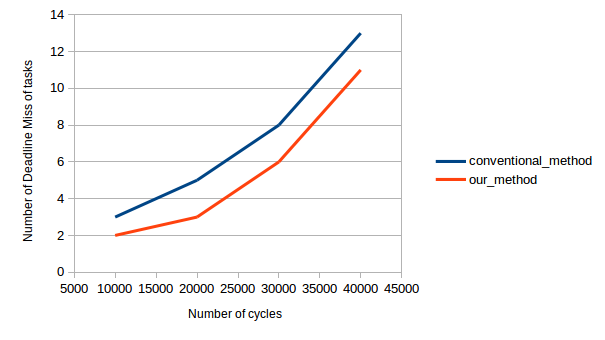
\includegraphics[width=12cm,height=7cm]{Graph_4.png}
}
\caption{Number of Task Misses on Dataset II for a memory with 19 banks and row size 32B over 40,000 cycles}
\end{figure}


\begin{figure}
%\label{fig1}
\centering
\fbox{
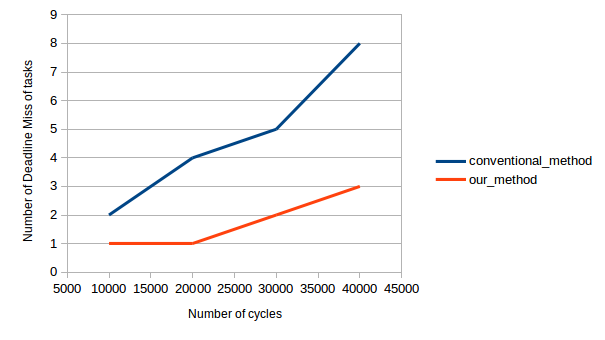
\includegraphics[width=12cm,height=7cm]{Graph_5.png}
}
\caption{Number of Task Misses on Dataset III for a memory with 15 banks and row size 64B over 40,000 cycles}
\end{figure}

\begin{figure}
%\label{fig1}
\centering
\fbox{
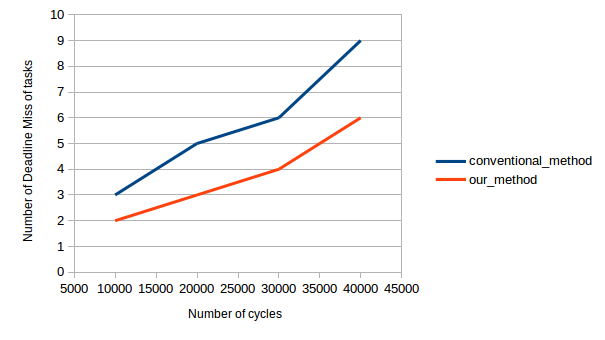
\includegraphics[width=12cm,height=7cm]{Graph_6.png}
}
\caption{Number of Task Misses on Dataset III for a memory with 15 banks and row size 32B over 40,000 cycles}
\end{figure}

\begin{figure}
%\label{fig1}
\centering
\fbox{
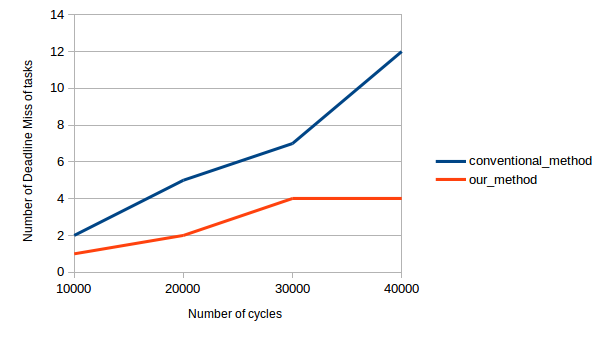
\includegraphics[width=12cm,height=7cm]{Graph_7.png}
}
\caption{Number of Task Misses on Dataset IV for a memory with 12 banks and row size 64B over 40,000 cycles}
\end{figure}

\begin{figure}
%\label{fig1}
\centering
\fbox{
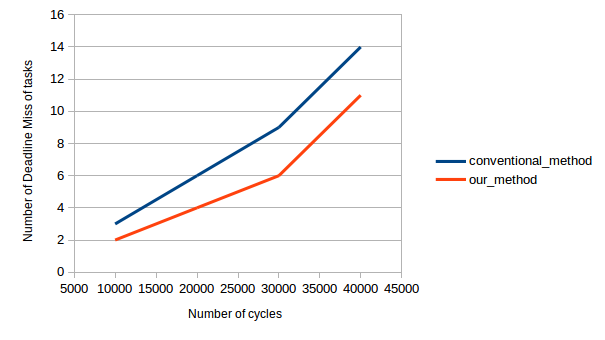
\includegraphics[width=12cm,height=7cm]{Graph_8.png}
}
\caption{Number of Task Misses on Dataset IV for a memory with 12 banks and row size 32B over 40,000 cycles}
\end{figure}




